\documentclass[a4paper,12pt,oneside]{report}
\usepackage{OvidiusFMI}
\usepackage{times}
\usepackage{graphicx}
\usepackage{hyperref}
\usepackage{color,xcolor}
\usepackage{amsmath}
\usepackage{framed}
\usepackage{indentfirst}
\usepackage{enumerate}
\usepackage[shortlabels]{enumitem}
\usepackage{listings}
\usepackage{amsmath,amsfonts,amssymb,amsthm,epsfig,epstopdf,url,array}
\usepackage{multicol,multirow}
\definecolor{code}{rgb}{0.97,0.97,0.97}
\lstdefinestyle{customc}{
  belowcaptionskip=1\baselineskip,
  backgroundcolor=\color{code},
  breaklines=true,
%  frame=L,
%  xleftmargin=\parindent,
  language=C,
  showstringspaces=false,
  morekeywords={bool,
  				 glutMainLoop, glutIdleFunc, glMatrixMode, glLoadIdentity, glPushMatrix, glPopMatrix, 
  				 glBegin, glEnd, glTranslatef, glRotatef, glScalef, glColor3f, glColor4f, glutSolidCube, glutWireCube, glutSolidSphere,
  				 glutWireSphere, glutSolidCone,glutSetWindowTitle,glutGet,glClear,glutSwapBuffers,glDepthFunc,
  				 glutWireCone, glutSolidTorus, glutWireTorus, glutSolidDodecahedron, glutWireDodecahedron,
  				 glutSolidOctahedron, glutWireOctahedron, glutSolidTetrahedron, glutWireTetrahedron, 
  				 glVertex3f,glVertex2f,glPointSize,
  				 glutSolidIcosahedron, glutWireIcosahedron, glutSolidTeapot, glutWireTeapot,glutReshapeFunc,
  				 glFlush, gluPerspective, glutPostRedisplay, glutInit, glutKeyboardFunc,glutKeyboardUpFunc,
  				 glutInitWindowSize, glutInitWindowPosition, glutInitDisplayMode, glutCreateWindow, glutDisplayFunc,glutPassiveMotionFunc,
  				 glClear,glTexCoord2f,
  				 glEnable, glDisable, glLightfv, glMaterialfv, glCullFace,glViewport,
  				 glFrontFace,glColor3ub, glShadeModel,
  				 glGenLists, glGetFloatv,glGentextures,glTexImage2D,glTexParameteri, free, glDeleteTextures,
  				 glLineStipple, glLineWidth, glBindTexture,glGenTextures,
  				 glNewList, glEndList, glCallList,
  				 glMap1f,glEvalCoord1f,glMapGrid1d,glEvalMesh1,glMap2f,glEvalCoord2f,glMapGrid2f,glEvalMesh2,
  				 gluBeginTrim, gluEndTrim, gluPwlCurve,glHint,
  				 GLUnurbsObj, gluBeginSurface, gluNurbsSurface, gluEndSurface, gluNewNurbsRenderer, 									gluNurbsProperty,gluQuadricNormals,
  				 glNormal3f,
  				 gluQuadricTexture,GLUquadricObj,gluSphere,
  				 glPolygonMode, glBlendFunc,glFogi,glFogiv,glFogfv,
  				 GLfloat, GLdouble, GLint,GLuint, GLushort,GLubyte, glRasterPos2f,
  				 gluBeginCurve, gluNurbsCurve, gluEndCurve,
  				 glOrtho, gluLookAt, glutBitmapCharacter, 
  				 glInitNames, glPushName, glLoadName, glSelectBuffer, glRenderMode,gluPickMatrix, glGetIntegerv, glutMouseFunc,glutMotionFunc,system,
  				 glPushAttrib, glPopAttrib, glMultMatrixf, sprintf, glClearStencil, glStencilFunc,glStencilOp,glStencilMask,glColorMask,glActiveStencilFaceEXT,fprintf},  
%   numbers=left,                    % where to put the line-numbers; possible values are (none, left, right)
  %numbersep=5pt,                   % how far the line-numbers are from the code
  %numberstyle=\tiny\color{code}, % the style that is used for the line-numbers
  basicstyle=\footnotesize\ttfamily,
  keywordstyle=\bfseries\color{green!40!black},
  commentstyle=\itshape\color{purple!40!black},
  identifierstyle=\color{blue},
  stringstyle=\color{orange},
}

\lstset{escapechar=@,style=customc}


\newtheorem{definition}{Defini\c tie}
\newtheorem{proposition}{Propozi\c tie}
\newtheorem{demonstration}{Demonstra\c tie}
\newtheorem{example}{Exemplu}
\newtheorem{theorem}{Teorem\u a}
\newtheorem{solve}{Rezolvare}
\newtheorem{corollary}{Corolar}

\facultatea{Matematic\u a \c si Informatic\u a}
\specializarea{Informatic\u a}
\teza{licen\c t\u a}
\titlu{Licen\c t\u a}
\coordonatorPrincipal{Cosma Lumini\c ta}
\autor{T\u anase Ramona Elena}
\data{2021}

\begin{document}
\maketitle

\pagenumbering{roman}
\tableofcontents

\pagenumbering{arabic}
%
%
%CAPITOLUL 1
%
%
\chapter{Definitii. Proprietati}

\section{Definitii. Proprietati}

Studiul funcțiilor convexe de o variabila reala, oferă o imagine excelentă a frumuseții și fascinației matematicii avansate. Vom găsi aici o mare varietate de rezultate bazate pe argumente simple și intuitive care au aplicații remarcabile.

In continuare vom nota cu I un interval nedegenerat din \(\mathbb{R}\).

\subsection{Definitie}

O functie \(f: I \rightarrow \mathbb{R}\) se numeste convexa daca,
\begin{displaymath}
f \left ( \left ( 1 - \lambda  \right )x + \lambda y \right )\leq \left ( 1 - \lambda  \right ) f_{\left ( x \right )} + \lambda f_{\left ( y \right )} 	\label{eq:1.1} \tag{1.1}
\end{displaymath}

pentru orice \(x\) si \(y\) din \(I\), si orice \(\lambda \in \left [ 0,1 \right ]\). Functia \(f\) se numeste strict convexa daca inegalitatea \ref{eq:1.1} se pastreaza  stricta pentru orice x si y din I, si orice  \(\lambda \in \left ( 0,1 \right )\) . Daca \(-f\) este convexa (respective stric convexa), atunci spunem ca \(f\) este concava (respectiv strict concava). Daca \(f\) este si convexa si concava, atunci spunem ca \(f\) este functie afina. 


Functiile afine sunt tocmai functiile de forma \(mx + n\),  \(m\) si \(n\) constante reale.
Se poate demonstra usor faptul ca urmatoarele trei functii sunt convexe (desi nu sunt strict convexe):
\begin{enumerate}
  \item partea pozitiva \(x^{+} = max \left \{ x,0 \right \}\),
  \item partea negative \(x^{-} = max \left \{ -x,0 \right \}\), 
  \item modulul \(\left | x \right | = max \left \{ -x,x \right \}\),
  \item functia patratica \(x^{2}\)  este strict convexa pe \(\mathbb{R}\),
  \item functia radacina patrata \(\sqrt{x}\) este strict concava pe \(\mathbb{R}_{+}\). 
\end{enumerate}

Alte criterii de convexitate legate de teoria de baza a functiilor convexe vor fi prezentate in cele ce urmeaza. 
Convexitatea unei functii \(f : I\rightarrow \mathbb{R}\), inseamna geometric faptul ca, punctele de pe graficului lui  \(f|_{\left [ u,v \right ]}\) sunt sub (sau pe) coarda care uneste capetele \(\left ( u , f {\left ( u \right )} \right )\)  si \(\left ( v , f {\left ( v \right )} \right )\), pentru orice \(u, v \in I, u < v\); 
Vezi Fig 1.1 . Astfel inegalitatea \ref{eq:1.1} este echivalenta cu 
\begin{displaymath}
  f\left ( x \right )\leq f\left ( u \right ) +\frac{f\left ( v \right )- f\left ( u \right )}{v - u}\left ( x - u \right ) \label{eq:1.2} \tag{1.2}
\end{displaymath}
pentru orice \(x\in \left [  u, v\right ]\), si \(u, v \in I, u < v\). 

\begin{center}
	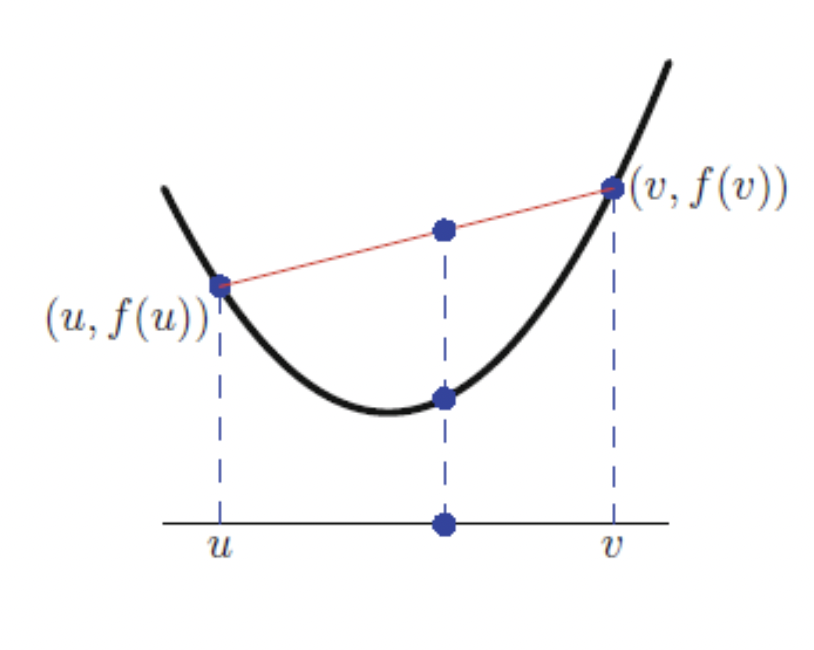
\includegraphics[width=0.5\textwidth]{fig1.1.png}
	\\ Fig 1.1 Frunctii convexe: graficul este sub coarda
\end{center}

Aceasta remarca arata faptul ca functiile convexe sunt majorate de functiile afine pe orice subinterval compact. 

Fiecare functie convexa f este marginita pe fiecare subinterval compact \(\left [ u , v \right ]\) a intervalului pe care este definita. De fapt , \(f\left ( x \right ) \leq  M = max \left \{ f\left ( u \right ), f\left ( v \right ) \right \}\)  pe \(\left [ u , v \right ]\)  si scriind un punct arbitrar \(x\in  \left [ u , v  \right ]\)  ca  \(x= \frac{\left ( u + v \right )}{2} + t\) pentru unii \(t\) cu \(\left | t \right |\leq \frac{\left ( v - u \right )}{2}\) , deducem cu usurinta ca 

\begin{displaymath}
  f\left ( x \right )=  f\left ( \frac{u+v}{2} + t\right )\geq 2 f\left ( \frac{u + v}{2} \right )- f\left ( \frac{u + v}{2} - t\right )\geq 2f\left ( \frac{u+v}{2} \right ) - M
\end{displaymath}

\subsection{Teorema}
O functie convexa \(f: I \rightarrow \mathbb{R}\) este continua in orice punct interior al lui \(I\). 	


\begin{demonstration}
	Presupunem ca \(a\in I\)
 si alegem \(\varepsilon > 0\)
 astfel incat \(\left [ a - \varepsilon , a + \varepsilon  \right ] \subset I\).
 Atunci  
\begin{displaymath}
  f\left ( a \right )\leq \frac{1}{2} f\left ( a - \varepsilon  \right ) + \frac{1}{2}f \left ( a + \varepsilon  \right )
\end{displaymath}
si 
\begin{displaymath}
  f\left ( a \pm t\varepsilon  \right )= f\left ( \left ( 1 - t \right ) a + t\left ( a \pm \varepsilon  \right )\right )\leq \left ( 1 - t \right )f\left ( a \right ) + tf\left ( a\pm \varepsilon  \right )
\end{displaymath}
pentru orice \(t\in \left [ 0 , 1 \right ]\). Prin urmare 
\begin{displaymath}
  t\left ( f\left ( a\pm \varepsilon  \right ) - f\left ( a \right ) \right )\geq f\left ( a\pm t\varepsilon  \right )- f\left ( a \right )\geq -t\left ( f\left ( a\mp \varepsilon  \right ) - f\left ( a \right )\right )
\end{displaymath}

care ne conduce la 

\begin{displaymath}
\left | f\left ( a\pm t\varepsilon  \right )- f\left ( a \right ) \right |\leq t max \left \{ \left | f\left ( a-\varepsilon  \right )- f\left ( a \right ) \right |, \left | f\left ( a+\varepsilon  \right ) - f\left ( a \right )\right | \right \},
\end{displaymath}
 pentru orice \(t\in \left [ 0 , 1 \right ]\). Continuitatea functiei \(f\) este acum clara. 
	Exemple simple precum, \(f\left ( x \right )= 0\) daca \(x\in \left ( 0 , 1 \right )\), si daca \(f\left ( 0 \right )= f\left ( 1 \right ) = 1\), arate faptul ca salturi in sus pot aparea la punctele finale ale intervalului de definire a unei functii convexe. Din fericire, aceste posibile discontinuitati pot fi inlaturate. 

\end{demonstration}

\subsection{Propozitie}
Daca \(f: \left [ a, b \right ]\rightarrow \mathbb{R}\) este o functie convexa, atunci limitele \(f\left ( a+ \right ) = \lim_{x\rightarrow a, x> a}f\left ( x \right )\)  si \(f\left ( b- \right ) = \lim_{x\rightarrow b, x< b}f\left ( x \right )\) exista in \(\mathbb{R}\) si
\begin{displaymath}
  \tilde{f}\left ( x \right )= \left\{\begin{matrix}
f\left ( a+ \right ) & \\ 
 f\left ( x \right )& \\ 
 f\left ( b- \right )& 
\end{matrix} \begin{matrix}
\text{daca } x=a & \\ 
\text{daca } x\in \left ( a,b \right ) & \\ 
\text{daca } x= b& 
\end{matrix}\right.
\end{displaymath}
 este o functie convexa continua. 

	Acest rezultat este o consecinta a urmatoarelor rezultate :

% Rescris folosind noul doc (15/11/21)

\subsection{Lema}

Daca \(f: I \rightarrow \mathbb{R}\) este convexa, atunci sau \(f\) este monotona pe intervalul \(I\), sau exista un punct \(\xi \in int I\) astfel incat \(f\) este descrescatoare pe intervalul \(\left ( -\infty , \xi  \right )\cap I\) si crescatoare pe intervalul \(\left[\xi , \infty  \right )\cap I\).

\begin{demonstration}
Luam \(a < b\) puncte interioare arbitrare ale lui \(I\) si fie 
\(m = inf\left \{ f\left ( x \right )  : x\in \left [ a,b \right ]\right \}\). Cum \(f\) este continua pe \(\left [ a,b \right ]\), acest infimum este atins in punctul \(\xi \in \left [ a,b \right ]\), adica 
\begin{displaymath}
  m = f\left ( \xi  \right )
\end{displaymath}
Daca \(a \leq x <  y< \xi\), atunci \(y\) este o combinatie convexa a lui \(x\) si \(\xi\), mai exact, \(y = \frac{\xi -y}{\xi -x}x + \frac{y - x}{\xi -x}\xi\). Cum \(f\) este convexa, 
\begin{displaymath}
  f\left ( y \right )\leq \frac{\xi -y}{\xi -x}f\left ( x \right )+ \frac{y-x}{\xi -x}f\left ( \xi  \right )\leq f\left ( x \right ) 
\end{displaymath}
Demonstratia se incheie cu un process de lipire (la stanga lui \(a\) si la dreapta lui \(b\)), observand ca proprietatea de covexitate face imposibila existent a trei numere \(u < v < w\) in \(I\) astfel incat \(f\left ( u \right ) < f\left ( v \right )> f\left ( w \right )\). 
\end{demonstration}

\subsection{Corolar}
\begin{enumerate}[a)]
\item Orice functie convexa \(f: I \rightarrow \mathbb{R}\) care nu este monotona pe
intervalul \(I\) are un minim global interior. 
\item Daca o functie convexa \(f: \mathbb{R} \rightarrow \mathbb{R}\) este marginita superior, atunci este constanta.
\end{enumerate}
Atingere supremului la capete nu este o proprietate caracteristica a functiilor convexe, dar insa avem urmatorul rezultat. 

\subsection{Teorema}

Fie \(f: I \rightarrow \mathbb{R}\). Atunci \(f\) este (strict) convexa daca si numai daca pentru orice subinterval compact \(J\) al lui \(I\), si fiecare functie afina \(L\), supremul lui \(f+L\) pe \(J\) este atins intr-un capat al intervalului (si doar acolo). 


\begin{demonstration}
Ne vom restrange la cazul functiilor convexe. Cazul functiilor strict convexe poate fi tratat in acelasi mod. 
\\ Necesitatea: Daca \(f\) este convexa, la fel este si suma \(F = f + L\). Cum orice punct al unui subinterval \(J = \left [ x , y \right ]\) este o combinatie convexa \(z = \left ( 1 - \lambda  \right )x + \lambda y \) a lui \(x\) si \(y\), avem
\begin{displaymath}
  \sup_{z\in J}F\left ( z \right ) = \sup_{\lambda \in \left [ 0 , 1 \right ]}F\left ( \left ( 1 - \lambda  \right )x + \lambda y \right )\leq \sup_{\lambda \in \left [ 0,1 \right ]}\left [ \left ( 1-\lambda  \right )F\left ( x \right ) + \lambda F\left ( y \right ) \right ] + max \left \{ F\left ( x \right ), F\left ( y \right ) \right \}
\end{displaymath}

Suficienta: Avand un subinterval \(J = \left [ x,y \right ]\) al lui \(I\), exista o functie afina \(L\left ( x \right ) = mx + n\) care este egala cu \(f\) la punctele  \(x\) si \(y\). 
Atunci
\begin{displaymath}
  \sup_{\lambda \in \left [ 0,1 \right ]}\left [ \left ( f - L \right )\left ( 1 - \lambda  \right )x + \lambda y \right ] = 0
\end{displaymath}

Care ne conduce la 
\begin{displaymath}
  0\geq f\left ( \left ( 1 - \lambda  \right )x + \lambda y \right )- L\left ( \left ( 1 - \lambda  \right )x - \lambda L \right )= f\left ( \left ( 1 - \lambda  \right )x + \lambda y  \right ) - \left ( 1 - \lambda  \right )L\left ( x \right ) - \lambda L\left ( y \right ) =
\end{displaymath}

\begin{displaymath}
  = f\left ( \left ( 1 - \lambda  \right )x + \lambda y \right ) - \left ( 1 - \lambda  \right ) f\left ( x \right ) - \lambda f \left ( y \right )
\end{displaymath}


Pentru orice \(\lambda \in \left [ 0,1 \right ]\). 

\end{demonstration}

\subsection{Remarca}

O functie \(f: I \rightarrow \mathbb{R}\) se numeste cvasiconvexa daca,
 \begin{displaymath}
  f\left ( \left ( 1-\lambda  \right )x + \lambda y \right )\geq  min\left \{ f\left ( x \right ), f\left ( y \right ) \right \}
\end{displaymath}
pentru orice  \(x, y \in I\) si \(\lambda  \in \left ( 0,1 \right ]\).
	 Urmatoarea caracterizare a convexitatii in cadrul clasei functiilor continue se dovedeste utila si in verificarea convexitatii. 

\subsection{Teorema}
O functie \(f : I \rightarrow \mathbb{R}\) este convexa daca si numai daca ea verifica urmatoarele doua conditii:
\begin{enumerate}[a)]
\item \(f\) este continua in fiecare punct din interiorul lui \(I\); si
\item \(f\) este convexa in punctul de mijloc , adica, 
\end{enumerate}

\begin{displaymath}
  f\left ( \frac{x+y}{2} \right )\leq \frac{f\left ( x \right )+f\left ( y \right )}{2}
\end{displaymath}
pentru orice \(x, y \in I\). 


\begin{demonstration}
Necesitatea rezulta din teorema 1.1.2. Suficienta este demonstrate prin reducerea la absurd. Daca \(f\) nu este convexa, atunci exista un interval \(\left [ a,b \right ]\) astfel incat graficul functiei \(f\) restricionata la  \(\left [ a,b \right ]\) sa nu fie sub coarda care uneste punctele \(\left ( a, f\left ( a \right ) \right )\) si \(\left ( b, f\left ( b \right ) \right )\); ca urmare , functia
\begin{displaymath}
  \varphi \left ( x \right )= -f\left ( x \right ) + f\left ( a \right )+ \frac{f\left ( b \right )- f\left ( a \right )}{b-a}\left ( x-a \right ), x\in \left [ a,b \right ]
\end{displaymath}
are  \(\gamma = inf \left \{ \varphi \left ( x \right ) : x\in \left [ a,b \right ]\right \}< 0\). Observam ca \(-\varphi\) este convexa in punctul de mijloc, continuu si \(\varphi \left ( a \right ) =\varphi \left ( b \right ) = 0\). Fie \(c = inf \left \{ x \in \left [ a,b  \right ] : \varphi \left ( x \right )= \gamma \right \} \), atunci \(\varphi \left ( c \right ) = \gamma\)  si \(c \in \left ( a,b  \right )\). Conform definitiei lui \(c\), pentru orice \(h>0\) pentru care \(c\pm h\in \left ( a,b \right )\) avem 
\begin{displaymath}
  \varphi \left ( c - h  \right )> \varphi \left ( c \right ) si \varphi \left ( c + h  \right )\geq  \varphi \left ( c \right )
\end{displaymath}

Astfel 
\begin{displaymath}
  -\varphi \left ( c \right )> \frac{-\varphi \left ( c-h \right )-\varphi \left ( c+h \right )}{2} 
\end{displaymath}
Ceea ce este in contraditie cu faptul ca \(-\varphi\) esteconvexa in punctul de mijloc. 
\end{demonstration}


\subsection{Corolar}

Fie \(f: I \rightarrow \mathbb{R}\) o functie continua. Atunci, \(f\) este convexa daca si numai daca
\begin{displaymath}
  f\left ( x+h \right )+ f\left ( x - h \right ) - 2f\left ( x \right )\geq 0
\end{displaymath}

pentru orice \(x \in I\) si orice \(h > 0\) astfel incat si \(x + h\) si \(x - h\) apartin lui \(I\). 
Observam ca si Teorema 1.1.8 si corolarul acesteia 1.1.9 de mai sus, admit variante in cazul functiilor strict convexe, 
Corolarul 1.1.9 ne permite sa verificam imedat convexitatea / concavitatea stricta a unor functii elementare, precum functia exponentiala, cea logaritmica, si restrictia functiei sinus pe \(\left [ 0 , \pi \right ]\). Intradevar, pentru functia exponentiala , faptul ca  \(a , b > 0, a\neq b\), implica \(\frac{a + b}{2}> \sqrt{ab}\)
este echivalenta cu 
\(e^{x + h} + e^{x - h } - 2e^{x}> 0\)
pentru orice \(x\in \mathbb{R}\) si orice \(h > 0\).
	Multe alte exemple pot fi deduse folosind urmatoarele proprietati ale functiilor convexe / concave. 

\subsection{Propozitie}
Operatii cu functii convexe 
\begin{enumerate}[a)]
\item Adunand doua functii convexe ( definite pe acelasi interval) obtinem o functie convexa; daca una dintre ele este strict convexa, atunci suma lor este de asemenea strict convexa.
\item Inmultind o functie (strict) convexa cu un scalar (strict)  pozitiv obtinem de asemenea o functie (strict) convexa.
\item Presupunem ca f si g sunt doua functii convexe pozitive definite pe un interval I. Atunci, produsul lor este o functie convexa pe I daca sunt sincrone in sensul ca, \begin{displaymath}
   \left ( f\left ( x \right ) - f\left ( y \right ) \right )\left ( g\left ( x \right ) - g\left ( y \right )\right )\geq 0
\end{displaymath} pentru orice \(x , y \in \mathbb{R}\); de exemplu , aceasta conditie apare daca f si g sunt amandoua descrescatoare sau amandoua crescatoare.
\item Restrictia unei functii (strict) convexe pe I, la un subinterval al lui I este de asemenea o functie (strict) convexa. 
\item Presupunem ca \(f\) este o functie bijectiva intre doua interval \(I\) si \(J\). Daca \(f\) este strict crescatoare, atunci \(f\) este (strict) convexa daca si numai daca \(f^{-1}\) este (strict) concava. Daca \(f\) este o functie bijectiva descrescatoare, atunci \(f\) si  \(f^{-1}\) sunt ambele convexe sau ambele concave.
\item Daca \(f\) este o functie strict pozitiva concava, atunci \(\frac{1}{f}\) este o functie convexa. Aici rolul concavitatii si al convexitatii nu poate fi schimbat unul cu celalalt.
\item Maximul a doua functii (stricte) convexe \(f , g : I \rightarrow \mathbb{R}\),
\begin{displaymath}
  max \left \{ f , g \right \}\left ( x \right )=  max \left \{ f\left ( x \right ), g\left ( x \right ) \right \}
\end{displaymath} este de asemenea o functie (strict) convexa.
\item Compunerea \(f\left ( ax + b \right )\), a unei functii \(f\) convexe si a unei functii afine \(ax+b\), este o functie convexa. 
\end{enumerate}

Detaliile sunt simple. 
In continuare , vom discuta extinderea inegalitatii convexitatii(1.1). In primul rand, observam faptul ca intervalele sunt inchise la combinatii convexe arbitrare, adica, 
\begin{displaymath}
  \sum_{ k= 1}^{n}\lambda _{k}x_{k} \in I
\end{displaymath}
pentru orice \(x_{1},......, x_{n} \in\)  si orice \(\lambda _{1},......, \lambda _{n} \in \left [ 0 , 1  \right ]\) cu \(\sum_{k = 1}^{n} \lambda _{k} = 1\). Acest lucru poate fi demonstrat prin inductie dupa \(n\). Cazul \(n=1\) este trivial, in timp ce \(n = 2\) rezulta din definitia unei multimi convexe. Presupunand faptul ca rezultatul este adevarat pentru toate combinatiile convexe cu cel mult \(n\geq 2\) puncte, sa trecem la cazul combinatiilor cu \(n + 1\) puncte, \(x = \sum_{k = 1}^{n + 1} \lambda _{k}x_{k}\). Cazul non-trivial este atunci cand toti coeficientii \(\lambda _{k}\) se afla in \(\left ( 0 , 1 \right )\). Dar in acest cacz , datorita ipotezei de inductie, x poate fi reprezentat ca o combinatie convexa de doua elemente ale lui \(I\), 
\begin{displaymath}
  x = \left ( 1 - \lambda _{n + 1} \right )\left ( \sum_{k = 1}^{n} \frac{\lambda _{k}}{1 - \lambda _{n + 1}} x_{k}\right ) + \lambda _{n + 1}x_{n + 1},
\end{displaymath}
prin urmare x apartine lui \(I\). 
	Remarca de mai sus asupra intervalelor are o echivalenta remarcabila pentru functiile convexe :

\subsection{Lema}
Cazul discret al inegalitatii lui Jensen
O functie cu valoari reala \(f\) definite pe un interval \(I\) este convexa daca si numai daca pentru orice puncte \(x_{1},.......,x_{n}\) din \(I\) si orice scalari \(\lambda _{1},.......,\lambda _{n}\) din \(\left [ 0 , 1 \right ]\) cu \(\sum_{k = 1}^{n}\lambda _{k}= 1\) avem, 
\begin{displaymath}
  f\left ( \sum_{k = 1}^{n} \lambda _{k}x_{k}\right )\leq \sum_{k = 1}^{n}\lambda _{k}f\left ( x_{k} \right ).
\end{displaymath}

Daca \(f\) este strict convexa, inegalitatea de mai sus este stricta daca punctele \(x_{k}\) nu sunt toate egale intre ele , si scalarii \(\lambda _{k}\) sunt toti pozitivi. 

\begin{demonstration}
Prima afirmatie rezulta prin inductie matematica. In ceea ce priveste cea de a doua afirmatie, presupunem ca functia \(f\) este strict convexa si 
\begin{displaymath}
  f\left ( \sum_{k = 1}^{n} \lambda _{k}x_{k}\right )=  \sum_{k = 1}^{n}\lambda _{k}f\left ( x_{k} \right ). \label{eq:1.3} \tag{1.3}
\end{displaymath}
pentru  punctele \(x_{1}, ........, x_{n} \in I\) si cativa scalari \(\lambda _{1}, ........, \lambda _{n} \in \left ( 0 , 1\right )\) cu suma egala cu \(1\). Daca \(x_{1}, ........, x_{n}\) nu sunt toti egali, multimea \(S = \left \{ k: x_{k}<  max \left \{ x_{1,....,x_{n}} \right \} \right \}\) va fi o submultime proprie a multimii  \(\left \{ 1,....,n \right \}\) si \(\lambda _{S} = \sum_{k \in S}^{}\lambda _{S} \in \left ( 0,1 \right )\). Cum \(f\) este strict convexa avem, 
\begin{displaymath}
  f\left ( \sum_{k=1}^{n}\lambda _{k}x_{k} \right ) = f\left ( \lambda _{S}\left ( \sum_{k\in S}^{}\frac{\lambda _{k}}{\lambda _{S}} x_{k}\right ) +\left ( 1-\lambda _{S} \right )\left ( \sum_{k\notin S}^{} \frac{\lambda _{k}}{1 - \lambda _{S}}x_{k}\right )\right ) < 
\end{displaymath}
  
\begin{displaymath}
  \lambda _{S}f\left ( \sum_{k\in S}^{}\frac{\lambda _{k}}{\lambda _{S}} x_{k}\right ) +\left ( 1 - \lambda _{S} \right )f\left ( \sum_{k\notin S}^{}\frac{\lambda _{k}}{1 - \lambda _{S}} x_{k}\right ) < 
\end{displaymath}
  
\begin{displaymath}
  \lambda _{S} \sum_{k\in S}^{}\frac{\lambda _{k}}{\lambda _{S}} f\left ( x_{k} \right ) +\left ( 1 - \lambda _{S} \right ) \sum_{k\notin S}^{}\frac{\lambda _{k}}{1 - \lambda _{S}}f\left ( x_{k} \right )= \sum_{k=1}^{n}\lambda _{k}f\left ( x_{k} \right ),
\end{displaymath}
  

care contrazice ipoteza noastra \ref{eq:1.3}. Astfel, toate punctele \(x_{k}\) ar trebui sa coincida.
\end{demonstration}

O consecinta imediata a lemei 1.1.11 (cand este aplicata functiei exponentiale) este urmatorul rezultat care extinde bine cunoscuta inegalitate AM-GM( adica inegalitatea dintre media aritmetica si cea geometrica).


\subsection{Teorema}
Forma ponderata a inegalitatii AM-GM
Daca \(x_{1},.......,x_{n}\in \left ( 0,\infty  \right ) si \lambda_{1},......,\lambda _{n} \in \left ( 0 , 1 \right ), \sum_{k = 1}^{n}\lambda _{k}= 1\), atunci
\begin{displaymath}
  \sum_{k = 1}^{n}\lambda _{k}x_{k}> x_{1}^{\lambda _{1}}\cdots x_{n}^{\lambda _{n}}
\end{displaymath}

In afara de cazul cand \(x_{1} = \cdots = x_{n}\). 
	Inlocuind \(x_{k}\) cu \(\frac{1}{x_{k} }\) in ultima inegalitate, obtinem 
\begin{displaymath}
  x_{1}^{\lambda _{1}}\cdots x_{n}^{\lambda _{n}}> \frac{1}{\sum_{k = 1}^{n}}\frac{\lambda _{k}}{x_{k}}
\end{displaymath}

in afara de cazul cand \(x_{1} = \cdots = x_{n}\). 
Asta reprezinta forma ponderata a inegalitatii mediei geometrice – mediei armonice (adica de inegalitatea GM-HM). 

Pentru \(\lambda _{1} = \cdots =\lambda _{n}= \frac{1}{n}\) recuperam inegalitatea obisnuita care afirma ca pentru orice \(x_{1},.....,x_{n}\) de numere positive, nu toate egale, avem

\begin{displaymath}
  \frac{x_{1}+.....+x_{n}}{n}> \sqrt[n]{x_{1}\cdots x_{n}}> \frac{n}{\left ( \frac{1}{x_{1}}+....+\frac{1}{x_{n}} \right )}. 
\end{displaymath}




\section{Inegalitatea lui Young si consecintele sale}

Urmatoarul caz special al formei ponderate a inegalitatii AM-GM este cunoscuta sub numele de inegalitatea lui Young:  
\begin{displaymath}
  ab \leq \frac{a^{p}}{p}+ \frac{b^{q}}{q},
\end{displaymath}
pentru orice \(a,b \geq 0\),
si de fiecare data cand  \(p,q \in \left ( 0 , 1 \right )\) cu \(\frac{1}{p}+\frac{1}{q} = 1\); egalitatea are loc daca si numai daca \(a^{p}= b^{q}\). Inegalitatea lui Young poate fi de asemenea obtinuta ca o consecinta a convexitatii stricte a functiilor exponentiale. De fapt 
\begin{displaymath}
  ab = e^{log_{a}b}= e^{\left (\frac{1}{p}  \right )log_{a}p+ \left ( \frac{1}{q} \right )log_{b}q}
\leq \frac{1}{p}e^{log_{a}p}+\frac{1}{q}e^{log_{b}q}= \frac{a^{p}}{p}+\frac{b^{q}}{q}
\end{displaymath}

pentru toti \(a,b>0\) cu \(a^{p}\neq b^{q}\). Inca un argument este oferit de studiul variatiei functiei diferentiale. 
\begin{displaymath}
  F\left ( a \right )= \frac{a^{p}}{p}+\frac{b^{q}}{q} - ab, a\geq 0
\end{displaymath}

unde \(b\geq 0\) este un paramentru. Aceatsa functie atinge punctul minim globa strict la \(a= b^{\frac{q}{p}}\), care ne conduce la \(F\left ( a \right )> F\left ( b^{\frac{q}{p}} \right ) = 0\) pentru orice \(a\geq 0, a\neq b^{\frac{q}{p}}\). 
	W.H.Young a dovedid de fapt  o inegalitate mult mai generala, pentru \(f\left ( x \right )=  x^{p-1}\).

\subsection{Teorema}

Inegalitatea lui Young
Presupunem prin absurd ca \(f: \left [ 0,\infty  \right ) \rightarrow \left [ 0,\infty  \right )\) este o functie continua strict crescatoare astfel incat \(f\left ( 0 \right )= 0\) si \(\lim_{x\rightarrow \infty }f\left ( x \right )= \infty\). Atunci 
\begin{displaymath}
  uv\leq \int_{0}^{u}f\left ( x \right )dx + \int_{0}^{v}f^{-1}\left ( y \right )dy
\end{displaymath}

pentru orice \(u,v\geq 0\), si egalitatea are loc daca si numai daca \( v = f\left ( u \right )\). 

\begin{center}
	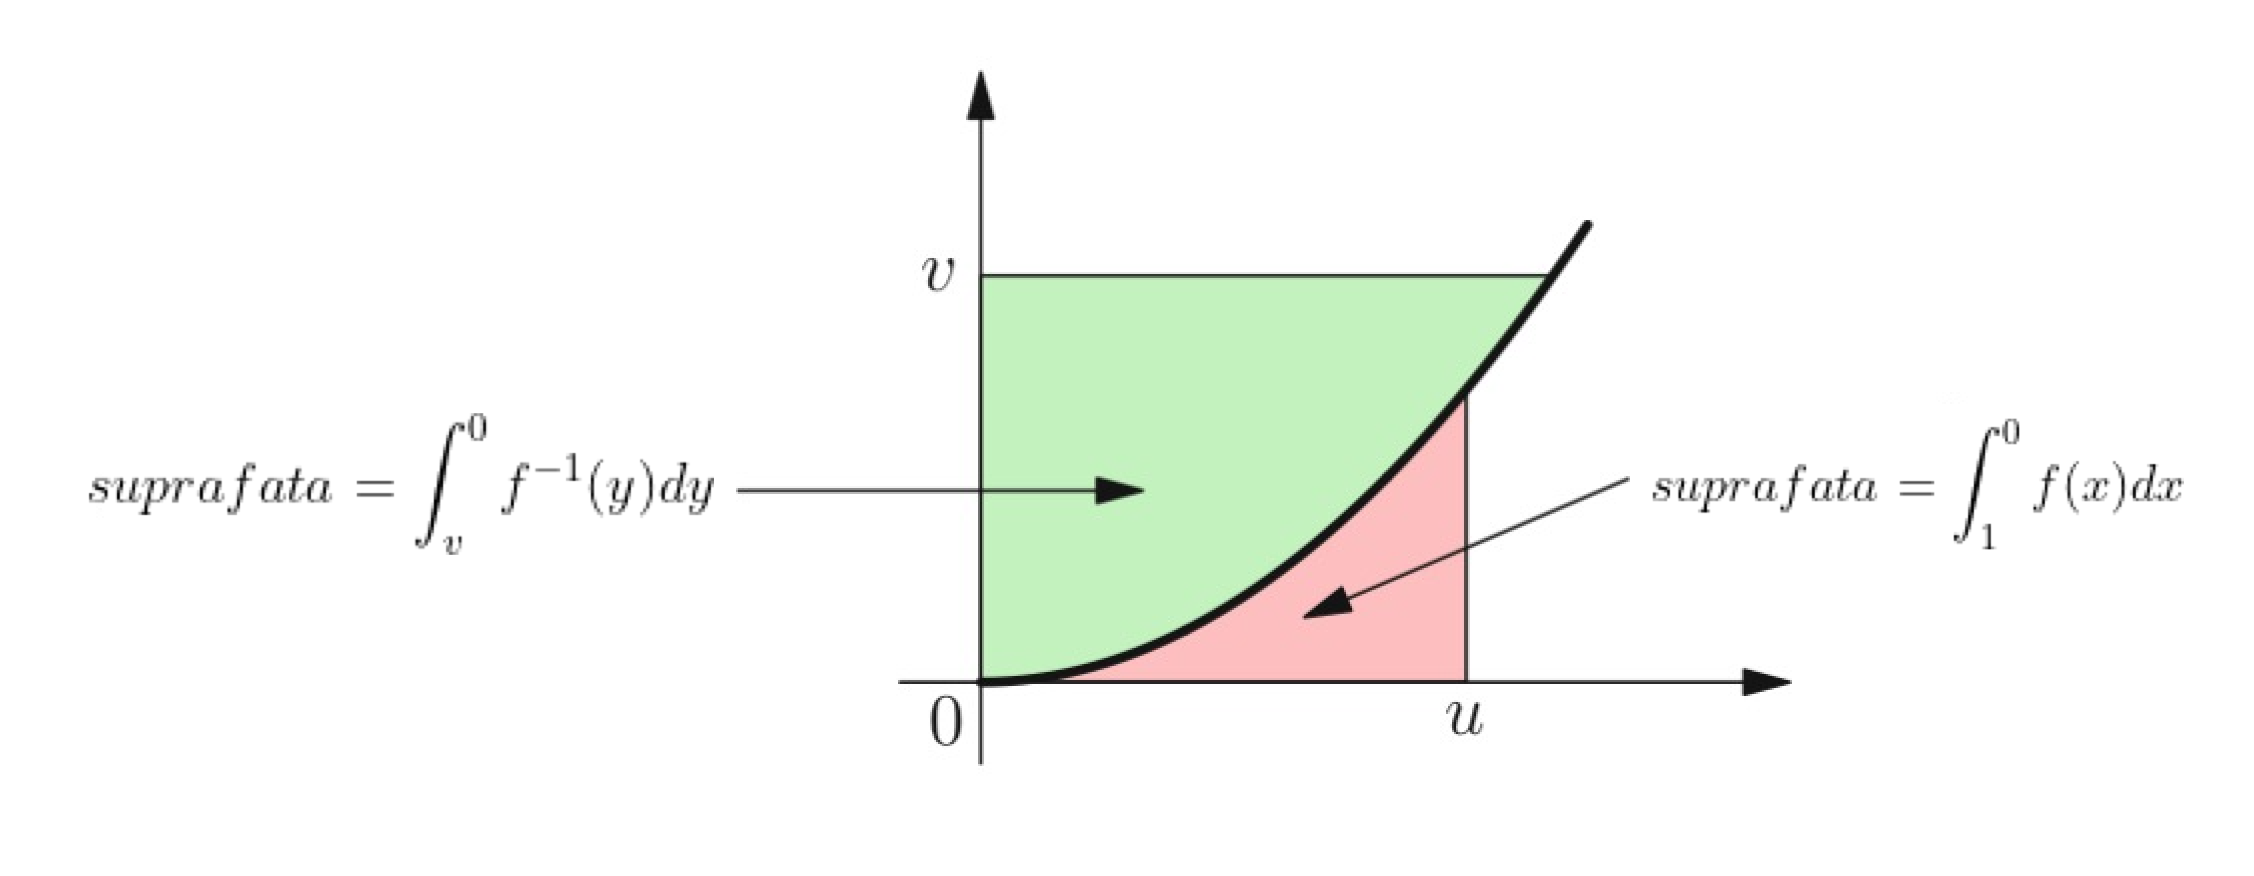
\includegraphics[width=1.0\textwidth]{fig1.2.png}
	\\ Fig 1.2
\end{center}

\begin{demonstration}
Folosind definitia derivatei se poate demonstra cu usurinta ca functia 
\begin{displaymath}
  F\left ( u \right )= \int_{0}^{u}f\left ( x \right )dx + \int_{0}^{f\left ( u \right )}f^{-1}\left ( y \right )dy -uf\left ( u \right ), u \in \left [ 0,\infty  \right )
\end{displaymath}

este diferentiala , cu \({F}'\) identic 0. Astfel, \(F\left ( u \right )= F\left ( 0 \right )= 0, pentru orice u\geq 0\). 
	Daca \(u, v \geq 0\)  si \(v\geq f\left ( u \right )\), atunci 
\begin{displaymath}
  uv = uf\left ( u \right )+ u\left ( v- f\left ( u \right ) \right )=  \int_{0}^{u}f\left ( x \right )dx + \int_{0}^{f\left ( u \right )}f^{-1}\left ( y \right )dy + u\left ( v - f\left ( u \right ) \right ) =
\end{displaymath}

\begin{displaymath}
  = \int_{0}^{u}f\left ( x \right )dx + \int_{0}^{v}f^{-1}\left ( y \right )dy + \left [ u\left ( v-f\left ( u \right )  \right ) - \int_{f\left ( u \right )}^{v}f^{-1}\left ( y \right )dy\right ]\leq 
\end{displaymath}

\begin{displaymath}
  \leq \int_{0}^{u}f\left ( x \right )dx + \int_{0}^{v}f^{-1}\left ( y \right )dy.
\end{displaymath}



	Cealalt caz, unde \(v\leq f\left ( u \right )\) poate fi tratat in acelasi mod. 
\end{demonstration}

\subsection{Teorema}

Inegalitatea lui Rogers-Hölder pentru p > 1

Fie \(p,q \in \left ( 1, \infty  \right )\) cu \(\frac{1}{p} + \frac{1}{q} = 1\), si  \(f\in L^{p}\left ( \mu  \right )\) si \(g\in L^{q}\left ( \mu  \right )\). Atunci \(fg\) apartine lui \(L^{1}\left ( \mu  \right )\) si avem 
\begin{displaymath}
  \left | \int_{\Omega}^{} fg  d\mu \right |\leq \int_{\Omega}^{}\left | fg \right |d\mu \label{eq:1.6} \tag{1.6}
\end{displaymath}

si 
\begin{displaymath}
  \int_{\Omega}^{}\left | fg \right |d\mu \leq \left \| f \right \|_{L^{p}}\left \| g \right \|_{L}^{q} . \label{eq:1.7} \tag{1.7}
\end{displaymath}

	Ca o consecinta 
\begin{displaymath}
  \left | \int_{\Omega}^{} fg  d\mu \right |\leq \left \| f \right \|_{L^{p}}\left \| g \right \|_{L}^{q}. \label{eq:1.8} \tag{1.8}
\end{displaymath}

	Rezultatul de mai sus se extinde intr-o maniera directa la perechi \(p = 1, q = \infty\) si \(p = \infty\). In domeniul complementar, \(p\in \left ( -\infty , 1 \right )\setminus \left \{ 0 \right \} si \frac{1}{p} + \frac{1}{q} = 1\), semnul inegalitatii in (1.6) – (1.8) ar trebui inversat. 
	Din Inegalitatea Rogers – Hölder rezulta ca pentru orice \(p, q, r \in \left ( 1 , \infty  \right )\) cu \(\frac{1}{p} + \frac{1}{q} = 1\) si orice \(f\in L^{p}\left ( \mu  \right )\) si \(g\in L^{q}\left ( \mu  \right )\) avem \(fg\in L^{r}\left ( \mu  \right )\) si 
\begin{displaymath}
  \left \| fg \right \|_{L^{r}}\leq \left \| f \right \|_{L^{p}}\left \| g \right \|_{L^{q}} \label{eq:1.9} \tag{1.9}
\end{displaymath}

%TODO REFS

Cazul de inegalitate de mai sus \ref{eq:1.8}, unde \(p = q = 2\), este cunoscut ca inegalitatea Cauchy-Bunyakovsky-Schwarz . 

\begin{demonstration}
Prima inegalitate este triviala. Daca \(f\) sau \(g\) sunt \(0 \mu\) – aproape peste tot, atunci cea de a doua inegalitate este triviala. Altfel, folosind inegalitatea lui Young, avem 
\begin{displaymath}
  \frac{\left | f\left ( x \right ) \right |}{\left \| f \right \|_{L^{p}}} \cdot \frac{\left | g\left ( x \right ) \right |}{\left \| g \right \|_{L^{q}}}\leq \frac{1}{p}\cdot \frac{\left | f\left ( x \right ) \right |^{p}}{\left \| f \right \|^{p}_{L^{p}}} + \frac{1}{q}\cdot \frac{\left | g\left ( x \right ) \right |^{q}}{\left \| g \right \|^{q}_{L^{q}}}.
\end{displaymath}
 
pentru orice \(x\) din \(\Omega\), astfel incat \(fg \in L^{1}\left ( \mu  \right )\). Prin urmare 
\begin{displaymath}
  \frac{1}{\left \| f \right \|_{L^{p}}\left \| g \right \|_{L^{1}}}\int_{\Omega }\left | fg \right |d\mu \leq 1.
\end{displaymath}
\end{demonstration}

\subsection{Remarca}

Conditii pentru egalitatea din Teorma 1.2.2
Observatia de baza este faptul ca  \(f\geq 0 si \int_{\Omega }f d\mu  = 0 implica f = 0 \mu-\) aproape peste tot. 
	Prin urmare avem egalitate in \ref{eq:1.6} daca si numai daca 
\begin{displaymath}
  f\left ( x \right )g\left ( x \right ) = e^{i\theta }\left | f\left ( x \right ) g\left ( x \right )\right |
\end{displaymath}
pentru o constanta reala \(\theta\) si pentru \(\mu-\) aproape peste toti \(x\). 
	Presupunem ca \(p , q \in \left ( 1 , \infty  \right )\) si \(f\) si \(g\) nu sunt zero \(\mu-\) aproape peste tot. Pentru a avea egalitate in \ref{eq:1.7} este necesar si suficient sa avem 
\begin{displaymath}
  \frac{\left | f\left ( x \right ) \right |}{\left \| f \right \|_{L^{p}}} \cdot \frac{\left | g\left ( x \right ) \right |}{\left \| g \right \|_{L^{q}}}\leq \frac{1}{p}\cdot \frac{\left | f\left ( x \right ) \right |^{p}}{\left \| f \right \|^{p}_{L^{p}}} + \frac{1}{q}\cdot \frac{\left | g\left ( x \right ) \right |^{q}}{\left \| g \right \|^{q}_{L^{q}}}. 
\end{displaymath}

\(\mu-\)aproape peste tot. Cazul egalitatii in Inegalitatea lui Young demonstreaza ca aceasta este echivalenta cu \(A\left | f\left ( x \right ) \right |^{p} = B\left | g\left ( x \right ) \right |^{q} \mu-\)aproape peste tot,
pentru unele numere positive A si B. 
	Daca \(p = 1\) si \(q = \infty\), avem egalitate in ecuatia \ref{eq:1.7} daca si numai daca avem o constanta \(\lambda \geq 0\) astfel incat \(\left | g\left ( x \right ) \right |\leq \lambda\),  \(\mu\) aproape peste tot, si \(\left | g\left ( x \right ) \right |= \lambda,  \mu\) aproape peste tot in multimea \(\left \{ x : f\left ( x \right )\neq 0 \right \}\). 

\subsection{Teorema}
Inegalitatea Minkowski
Pentru \(1\leq  p < \infty si f , g \in L^{p}\left ( \mu  \right ) \)avem
\begin{displaymath}
  \left \| f + g  \right \|_{L^{p}}\leq \left \| f \right \|_{L^{p}} + \left \| g \right \|_{L^{p}} \label{eq:1.10} \tag{1.10}
\end{displaymath}

\begin{demonstration}
Pentru \(p  = 1\), inegalitatea \ref{eq:1.10} rezulta imediat prin integrarea inegalitatii \(\left | f + g \right |\leq \left | f \right | + \left | g \right |\). Pentru \(p \in \left ( 1 , \infty  \right )\) avem:
\begin{displaymath}
  \left | f + g  \right |^{p}\leq \left ( \left | f \right | +\left | g \right |\right )^{p}\leq \left ( 2 sup\left \{ \left | f \right |,\left | g \right | \right \} \right )^{p}\leq 2^{p}\left ( \left | f \right |^{p}  + \left | g \right |^{p}\right )
\end{displaymath}
care ne demonstreaza ca \(f + g \in L^{p}\left ( \mu  \right )\). Mai mult de atat, conform Teoremei 1.2.2, 
\begin{displaymath}
  \left \| f + g  \right \|_{L^{p}}^{p} = \int_{\Omega }\left | f + g \right |^{p}d\mu \leq \int_{\Omega }\left | f + g \right |^{p - 1}\left | f \right |d\mu + \int_{\Omega }\left | f + g  \right |^{p - 1}\left | g \right |d\mu \leq 
\end{displaymath}

\begin{displaymath}
  \leq\left ( \int_{\Omega }\left | f \right |^{p}d\mu  \right )^{\frac{1}{p}}\left ( \int_{\Omega }\left | f + g  \right | ^{\left ( p - 1 \right )}d\mu \right )^{\frac{1}{q}}+ \left ( \int_{\Omega }\left | g \right |^{p}d\mu  \right )^{\frac{1}{p}}\left ( \int_{\Omega} \left | f + g \right |^{\left ( p - 1 \right )q}d\mu \right )^{\frac{1}{q}}= 
\end{displaymath}

\begin{displaymath}
  =\left ( \left \| f \right \|_{L^{p}} + \left \| g \right \|_{L^{p}} \right )\left \| f + g  \right \|_{L^{p}}^{\frac{p}{q}}
\end{displaymath}



unde \(\frac{1}{p} + \frac{1}{q} = 1\), si observam ca \(p - \frac{p}{q} = 1\). 	
\end{demonstration}


\subsection{Remarca}

Daca \(p = 1\), obtinem egalitate in \ref{1.10} daca si numai daca exista o functie masurabila pozitiva \(\varphi\) astfel incat 
\begin{displaymath}
  f\left ( x \right )\varphi \left ( x \right ) = g\left ( x \right )
\end{displaymath}
\(\mu –\) aproape peste tot in multimea \(\left \{ x : f\left ( x \right )g\left ( x \right )\neq 0 \right \}\). 
	Daca \(p \in \left ( 1 , \infty  \right )\) si \(f\) nu este o aproape peste tot, atunci avem egalitate in (1.10) daca si numai daca  \(g = \lambda f\) aproape peste tot, pentru unele \(\lambda \geq 0\). 
	In  cazul particular unde \(\left ( \Omega , \Sigma, \mu \right )\) este spatiul de masura asociat cu masura de numarare pe o muktime finite, \(\mu  : \rho \left ( \left \{ 1,......, n \right \} \right )\rightarrow \mathbb{N}, \mu \left ( A \right ) = \left | A \right |\), 
recuperam formele clasice discrete ale inegalitatilor de mai sus. De exemplu, poate fi citita versiunea discreta a inegalitatii lui Rogers- Holder
\begin{displaymath}
  \left | \sum_{k=1}^{n} \xi _{k}\eta _{k}\right |\leq \left ( \sum_{k = 1}^{n}\left | \xi _{k}\right |^{p}  \right )^{\frac{1}{p}}\left ( \sum_{k = 1}^{n} \left | \eta _{k} \right |^{q}\right )^{\frac{1}{q}}
\end{displaymath}

pentru  orice \(\xi _{k}, \eta _{k} \in \left \{ 1,.....,n \right \}.\) Pe de alta parte, un moment de reflectie demonstreaza faptul ca putem trece imediat de la aceste inegalitati discrete la analogiile lor integrale, corespunzatoare spatiilor de masura finite. 

\subsection{Remarca}

Mai multe despre inegalitatea Cauchy – Bunyakovsky – Schwarz
A.L. Cauchy , in faimosul sau curs de Analiza, a derivat cazul discret al acestei inegalitati din inegalitatea algebrica a  lui Lagrange ,
\begin{displaymath}
  \left ( \sum_{k = 1}^{n} a_{k}^{2}\right )\left ( \sum_{k = 1}^{n} b_{k}^{2}\right ) =  \sum_{1\leq j\leq k\leq n}\left ( a_{j}b_{k} - a_{k}b_{j} \right )^{2} + \left ( \sum_{k = 1}^{n} a_{k}b_{k}\right )^{2}
\end{displaymath}

Astfel 

\begin{displaymath}
  \left | \sum_{k = 1}^{n} a_{k}b_{k} \right |\leq \left ( \sum_{k = 1}^{n}a_{k}^{2} \right )^{\frac{1}{2}}\left ( \sum_{k = 1}^{n}b_{k}^{2} \right )^{\frac{1}{2}}
\end{displaymath}

pentru orice numere reale \(a_{1},.....,a_{n}, b_{1},......, b_{n}\). Cazul egalitatii este simplu. Inegalitatea corespunzatoare pentru integrale a fost demonstrate independent de V.Y.Bunyakovsky si H.A.Schwarz. 
	In 1890, H.Poincare a observant versiunea integrala a identitatii algebrice lui Lagrange (care da inegalitatea Cauuchy-Bunyakovsky-Schwarz in deplina generalitate ): Daca \(\mu\) este o masura de probabilitate pe un spatiu \(\Omega\) si \(f\) si \(g\) sunt doua functii apartinand spatiului \(L^{2}\left ( \mu  \right )\), atunci 
\begin{displaymath}
  \left (\int_{\Omega}f^{2}d\mu \right )\left (\int_{\Omega}g^{2}d\mu \right ) - \left (\int_{\Omega}fgd\mu \right )^{2} = \frac{1}{2}\int_{\Omega}\int_{\Omega}\left ( f\left ( x \right )g\left ( y \right ) - f\left ( y \right )g\left ( x \right )\right )^{2}d\mu \left ( x \right )d\mu \left ( y \right ).
\end{displaymath}
	El a folosit aceasta identitate integral pentru a deriva cazul unidimensional al unei inegalitati purtandu-i numele . O alta dovada simpla a inegalitatii Cauuchy-Bunyakovsky-Schwarz este oferita pntrintr-o identitat echivalenta cu legea cosinusurilor : pentru fiecare pereche de vectori nenuli \(x\) si \(y\) intr-un spatiu vectorial interior real, 
\begin{displaymath}
  \left \| \frac{x}{\left \| x \right \|} - \frac{y}{\left \| y \right \|}\right \|^{2} = 2 - 2\frac{\left \langle x , y \right \rangle}{\left \| x \right \|\left \| y \right \|}. 
\end{displaymath}



%
%
%CAPITOLUL 2
%
%


\chapter{Exercitii}

Multe dintre funcțiile familiare ale trigonometriei și geometriei au proprietăți de convexitate ușor de stabilit și, de cele mai multe ori, aceasta convexitatea are consecinţe utile.
Problema 1 (Pe maximul produsului a două muchii)
Într-un triunghi echilateral cu aria A, produsul dintre oricare două laturi este egal cu \(\left (\frac{4}{\sqrt{3}}  \right )\)A. Arătați că acesta reprezintă cazul extrem ceea ce inseamnca că, pentru un triunghi cu aria A trebuie să existe două laturi lungimile dintre care au un produs care este cel puțin la fel de mare ca \(\left (\frac{4}{\sqrt{3}}  \right )A\).
	Pentru a începe, avem nevoie de formule care să relaționeze lungimile marginilor cu zonele, și, în notația tradițională din figura 2.1, există trei formule egale în mod egal:

\begin{displaymath}
  A = \frac{1}{2}ab sin\gamma = \frac{1}{2}ac sin \beta = \frac{1}{2}bc sin \alpha. 
\end{displaymath}

\begin{center}
	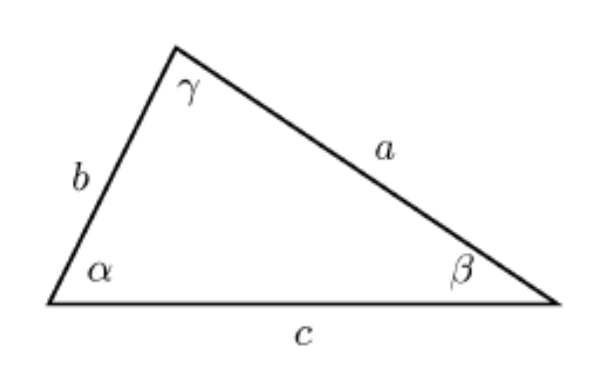
\includegraphics[width=0.5\textwidth]{fig2.1.png}
\end{center}

Fig. 2.1 Toate funcțiile trigonometrice sunt convexe (sau concave) dacă
Argumentele lor sunt limitate la un domeniu adecvat și, în consecință,
există multe consecințe geometrice interesante ale inegalității lui Jensen.

Aria A a triunghiului generic are trei reprezentari de baza :
\(A = \frac{1}{2}ab sin\gamma = \frac{1}{2}ac sin \beta = \frac{1}{2}bc sin \alpha. \)
Acum, dacă facem media acestor reprezentări, atunci găsim ca :
\begin{displaymath}
  \frac{1}{3}\left ( ab + ac + bc \right )= \left ( 2A \right )\frac{1}{3}\left \{ \frac{1}{sin \alpha } + \frac{1}{sin \beta } + \frac{1}{sin \gamma }\right \}, \label{eq:2.1.1} \tag{2.1.1}
\end{displaymath}

și aceasta este o formulă care aproape că ne imploră să întrebăm despre convexitatea \(\frac{1}{sin x}\). Reprezentarea grafica pentru \(x \mapsto \frac{1}{sin x}\), pentru \(x\in \left ( 0 , \infty  \right )\) cu siguranță este convexă, iar suspiciunile noastre pot fi confirmate prin calcularea derivatei a doua, \({\left ( \frac{1}{sin x} \right )}''= \frac{1}{sin x} + 2\frac{cos^{2}x}{sin ^{3}x}> 0\) pentru orice \(x\in \left ( 0, \pi  \right ) . (2.1.2)\)
	Prin urmare, din moment ce avem \(\frac{\left ( \alpha + \beta  + \gamma  \right )}{3}= \frac{\pi }{3}\), rezulta din inegalitatea lui Jensen ca 
\begin{displaymath}
  \frac{1}{3}\left \{ \frac{1}{sin \alpha }  + \frac{1}{sin \beta } + \frac{1}{sin \gamma }\right \}\geq \frac{1}{sin \frac{\pi }{3}} =  \frac{2}{\sqrt{3}}, 
\end{displaymath}

deci , prin inegalitatea (2.1.1), obtinem limita presupusa. 
m\begin{displaymath}
  ax \left ( ab, ac, bc \right )\geq \frac{1}{3}\left ( ab + ac + bc \right )\geq \frac{4}{\sqrt{3}}A \label{eq:2.1.3} \tag{2.1.3}
\end{displaymath}

Conexiuni si rafinamente 
Această problemă de provocare este strâns legată de o inegalitate binecunoscută a lui Weitzenböck care afirmă că în orice triunghi avem 
\begin{displaymath}
  a^{2} + b^{2} + c^{2} \geq \frac{4}{\sqrt{3}}A . \label{eq:2.1.4} \tag{2.1.4}
\end{displaymath}

De fapt, pentru a trece de la limita \ref{eq:2.1.3} la inegalitatea lui Weitzenböck trebuie doar să ne amintim ca 
\begin{displaymath}
  ab + ac + bc \leq a^{2} + b^{2} + c^{2}, 
\end{displaymath}

care este un lucru familiar pe care il putem obtine in trei moduri  - Inegalitatea lui Cauchy, limita AM-GM sau inegalitatea de rearanjare -  toți vor face acest lucru cu aceeasi grație.
	Inegalitatea lui Weitzenböck se dovedește a avea multe dovezi instructive - Engel (1998) dă unsprezece! 

Există câteva metode matematice pe care le-am putea numi generic amelioratori; în linii mari, acestea sunt metode care pot fi utilizate într- un mod semi-automat pentru a generaliza o identitate, de a rafina o inegalitate sau în caz contrar, sa îmbunătățeasca un rezultat dat. 
Următoarea problemă de provocare oferă un exemplu de alt fel. Aceasta sugerează cum s-ar putea gândi la ascuțirea aproape a oricărui rezultat care se obține prin inegalitatea lui Jensen.
Problema 2
Formula defectului lui Hölder
Daca \(f : \left [ a,b  \right ] \to \mathbb{R}\) este derivata de doua ori si daca vem limitele 
\begin{displaymath}
  0 \leq m \leq  f''\left ( x \right ) \leq  M , pentru orice x\in \left [ a,b \right ], \label{eq:2.2.1} \tag{2.2.1}
\end{displaymath}

atunci pentru orice valori reale \(a\leq x_{1}\leq x_{2}\leq ....\leq x_{n} \leq b \)si orice numere reale pozitive \(p_{k}, k= 1,2,.....,n  cu p_{1} + p_{2} + .....+ p_{n} = 1\), atunci axista o vaoare reala \(\mu \in \left [ m, M \right ]\) pentru care, una are formula
\begin{displaymath}
  \sum_{k = 1}^{n}p_{k}f\left ( x_{k} \right ) - f\left ( \sum_{k = 1}^{n} p_{k}x_{k}\right ) = \frac{1}{4}\mu \sum_{j = 1}^{n}\sum_{k = 1}^{n}p_{j}p_{k}\left ( x_{j} - x_{k} \right )^{2}. \label{eq:2.2.2} \tag{2.2.2}
\end{displaymath}

Acest rezultat provine din aceeași lucrare faimoasă din 1885 a lui Otto Ludwig Hölder (1859 1937) în care se găseşte dovada sa a inegalităţii care are a ajuns să fie cunoscută universal ca ”inegalitatea lui Holder”. Formula defectului \ref{eq:2.2.2} este mult mai puțin cunoscută, dar este totuși valoroasă. Aceasta oferă o măsură perfect naturală a diferenței dintre cele două părți ale inegalității lui Jensen și ne spune cum să învingem versiunea  inegalității lui Jensen ori de câte ori putem verifica ipoteza suplimentară \ref{eq:2.2.1}. 
În mod similar, dacă M este mic, să spunem \(0 \leq M \leq \epsilon\), atunci limita (2.2.1) ne spune că f se comportă mai degrabă ca o funcție afină \(f\left ( x \right ) = \alpha  + \beta x\). Pentru o funcție exact afină, partea stângă a limitei (2.2.1) este identic egal cu zero, dar în general limita \ref{eq:2.2.1} afirmă a relație mai subtilă. Mai precis, ne spune că partea stângă este un mic multiplu al unei măsuri de amploare  în care valorile \(x_{j}, j = 1,2,.....,n \)sunt difuzate pe tot intervalul \(\left [ a, b \right ]. \)

Această problemă ne duce in mod firesc la urmatoarea intrebar: Cum putem folosi faptul că \(0\leq m\leq {f}''\left ( x \right )\leq M \)? Odata c ne-am adresat intrebarea aceasta , s-ar putea să nu fie nevoie de mult pentru a observa că cele două funcții aferente
\begin{displaymath}
  g\left ( x \right ) = \frac{1}{2}Mx^{2} - f\left ( x \right ) si 
h\left ( x \right ) = f\left ( x \right ) - \frac{1}{2}mx^{2}
\end{displaymath}

sunt din nou convexe . In schimb aceasta observatie ne indeamna sa ne intrebam ce spune inegalitatea lui Jensen despre aceste functii. 
	Pentru \(g\left ( x \right )\), inegalitatea lui Jensen ne da limita 
\begin{displaymath}
  \frac{1}{2}M\bar{x}^{2} - f\left ( \bar{x} \right )\leq \sum_{k = 1}^{n}p_{k}\left \{ \frac{1}{2}Mx_{k}^{2} - f\left ( x_{k} \right )\right \}
\end{displaymath}

unde avem multimea \(\bar{x} = p_{1}x_{1}+ p_{2}x_{2}+ ..... + p_{n}x_{n}\) si aceasta limita este usor rearanjata pentru a duce la 
\begin{displaymath}
  \left \{ \sum_{k = 1}^{n} p_{k}f\left ( x_{k} \right )\right \} - f\left (\bar{x}  \right )\leq \frac{1}{2}M\left \{ \left ( \sum_{k=1}^{n} p_{k}x_{k}^{2}\right ) - \bar{x}^{2} \right \} = \frac{1}{2}M\sum_{k = 1}^{n}p_{k}\left ( x_{k} - \bar{x} \right )^{2}. 
\end{displaymath}

	Calculul analog pentru  \(h\left ( x \right )\) ne ofera o limita inferioara 
\begin{displaymath}
  \left \{ \sum_{k = 1}^{n} p_{k}f\left ( x_{k} \right )\right \} - f\left (\bar{x}  \right )\geq \frac{1}{2}m\sum_{k = 1}^{n}p_{k}\left ( x_{k} - \bar{x} \right )^{2}
\end{displaymath}

si aceste limite superioare si inferioare aproape completeaza demonstratia asertiei ( 2.2.1). Singurul lucru care lipseste este identitatea 
\begin{displaymath}
  \sum_{k = 1}^{n}p_{k}\left ( x_{k} - \bar{x} \right )^{2} = \frac{1}{2}\sum_{j = 1}^{n}\sum_{k = 1}^{n} p _{j}p_{k}\left ( x_{j} - x_{k} \right )^{2}
\end{displaymath}

care se poate verifica usor prin expansiunea algebrica si definirea lui \(\bar{x}\). 
	Comvexitatea si inegalitatea lui Jensen ofera solutii simple pentru multe probleme.  
	Urmatoarea problema vine din celebra sectiune cu probleme a ”American Mathematical Monthly” si ofera un exemplu clasic al acestui fenomen. 
	La inceput problema pare destul de usoara, dar, curand, intampinam dificultati. 

Problema 3(6)


\bibliographystyle{unsrt}
\setlength{\baselineskip}{\normalbaselineskip}
\setlength{\parskip}{0pt}
\bibliography{refs}
\end{document}